	
	\paragraph{QuizziPedia::Front-End::Index}
	\begin{figure} [ht]
		\centering
		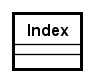
\includegraphics[scale=0.80]{UML/Classi/Front-End/QuizziPedia_Front-end_Views_Index.png}
		\caption{QuizziPedia::Front-End::Views::Index}
	\end{figure} \FloatBarrier
	\begin{itemize}
		\item \textbf{Descrizione}: \textit{view\ped{G}} generale dell'applicazione;
		\item \textbf{Utilizzo}: contiene gli elementi che saranno presenti in ogni pagina dell'applicazione;
		\item \textbf{Relazioni con altre classi}:
		\begin{itemize}
			\item \textbf{IN} \texttt{AppRun}: classe che verifica se l'utente sia autenticato e che abbia le giuste autorizzazioni per la pagina in cui si trova;
			\item \textbf{IN} \texttt{MenuBarDirective}: rappresenta il menù, presente in ogni pagina dell'applicazione, generato in base agli oggetti passati nello \$scope isolato. Fornisce un pulsante per ogni oggetto ricevuto come parametro, ogni pulsante viene rappresentato con un’icona e con un testo. Al click di un pulsante viene invocata la funzione ad esso associata;
			\item \textbf{IN} \texttt{FooterDirective}: \textit{directive\ped{G}} che mostra il footer dell'applicazione che sarà presente in ogni pagina;
			\item \textbf{IN} \texttt{ClickableAreaQuestionsView}: \textit{view\ped{G}} contenente i campi e le direttive per creare una domanda ad area cliccabile;
			\item \textbf{IN} \texttt{ConnectionQuestionsView}: \textit{view\ped{G}} contenente i campi e le direttive per creare una domanda a collegamento;
			\item \textbf{IN} \texttt{CreateQuestionnaireView}: \textit{view\ped{G}} per la creazione del questionario. In questo componente viene permesso anche all'utente di:
			\begin{itemize}
				\item Effettuare delle ricerche sul database di domande;
				\item Selezionare le domande da inserire nel questionario;
				\item Mostrare le domande già inserite e permettere all'utente di eliminarle da tale lista.
			\end{itemize}
			\item \textbf{IN} \texttt{EditorQMLView}: \textit{view\ped{G}} contenente l'editor QML per la creazione di domande personalizzate;
			\item \textbf{IN} \texttt{FillingQuestionnaireView}: \textit{view\ped{G}} principale per la compilazione del questionario; conterrà i vari templates di ogni domanda appartenente al questionario;
			\item \textbf{IN} \texttt{FilligQuestionsView}: \textit{view\ped{G}} contenente i campi e le direttive per creare una domanda a riempimento testo;
			\item \textbf{IN} \texttt{HomeView}: \textit{view\ped{G}} contenente la direttiva per barra di ricerca degli utenti e questionari e il bottone che porterà l'utente nella modalità allenamento;
			\item \textbf{IN} \texttt{ImagesSortingQuestionsView}: \textit{view\ped{G}} contenente i campi e le direttive per creare una domanda a ordinamento immagini;
			\item \textbf{IN} \texttt{LoginView}: \textit{view\ped{G}} contenente le form necessarie per effettuare il login. Contiene inoltre un link alla pagina di registrazione e uno alla pagina per il recupero della password;
			\item \textbf{IN} \texttt{MultipleQuestionsView}: \textit{view\ped{G}} contenente le direttive per creare una domanda a risposta multipla;
			\item \textbf{IN} \texttt{OtherUserView}: \textit{view\ped{G}} contenente le direttive dei dati personali e delle statistiche di un utente ricercato;
			\item \textbf{IN} \texttt{PasswordForgotView}: \textit{view\ped{G}} contenente le form necessarie per il recupero della password dimenticata; 
			\item \textbf{IN} \texttt{ProfileManagementView}: \textit{view\ped{G}} contenente i dati personali che un utente può modificare dopo essersi registrato al sistema;
			\item \textbf{IN} \texttt{QuestionnaireManagementView}:  \textit{view\ped{G}} principale per la gestione dei questionari;
			\item \textbf{IN} \texttt{QuestionsManagementView}: \textit{view\ped{G}} contenente l'elenco delle domande create; 
			\item \textbf{IN} \texttt{RegistrationManagementView}: \textit{view\ped{G}} che permette di visualizzare gli utenti iscritti ad un questionario;
			\item \textbf{IN} \texttt{ResultsQuestionnaireView}: \textit{view\ped{G}} contenente i risultati conseguiti dagli utenti che hanno compilato il proprio questionario;
			\item \textbf{IN} \texttt{ResultsView}: \textit{view\ped{G}} contenente i risultati della ricerca effettuata. Vengono visualizzati sia gli utenti che i questionari trovati;
			\item \textbf{IN} \texttt{SignUp}:  \textit{view\ped{G}} contenente le form dedicate alla registrazione utente. Contiene inoltre un link alla pagina di login;
			\item \textbf{IN} \texttt{StringSortingQuestionsView}:  \textit{view\ped{G}} contenente i campi e le direttive per creare una domanda a ordinamento stringhe; 
			\item \textbf{IN} \texttt{TrainingView}: \textit{view\ped{G}} principale della modalità allenamento; conterrà i vari templates di ogni domanda dell'allenamento;
			\item \textbf{IN} \texttt{TrueFalseQuestionsView}: \textit{view\ped{G}} contenente le direttive per creare una domanda vero/falso;
			\item \textbf{IN} \texttt{UserView}:  \textit{view\ped{G}} contenente le direttive dei dati personali dell'utente, delle sue statistiche relative ai questionari e agli allenamenti effettuati e dei questionari a cui è iscritto.
		\end{itemize}
	\end{itemize}
